\documentclass[fontset=none]{ctexart}
\ctexset{fontset=windows} %指定字体库为windows

\usepackage{fancyhdr}
\usepackage{fancyhdr}
\usepackage{ctex}
\usepackage{float}
\usepackage{amsmath,amsthm,amssymb,amsfonts}
\usepackage[left=3cm,right=3cm,top=2.5cm,bottom=2.5cm]{geometry}
\usepackage{graphicx}
\usepackage{epstopdf}
\usepackage{subfigure}
\pagestyle{fancy}%清除原页眉页脚样式

\fancyhead[R]{作者:姜鱼}
\fancyhead[C]{兼听则明,偏听则暗}

\begin{document}
  
    定义上,\textbf{设函数$f(x)$在$x=a$处的某一去心邻域内有定义,对于$\forall \varepsilon >0$,若$\exists \delta >0$,使得当$x$满足$0<\left| x-a \right|<\delta$时,都有$\left| f(x)-A \right|<\epsilon$,则称当x趋于a时,$f(x)$有极限A,记为$$\lim_{x \to 0}f\left( x \right) =A$$}


    极限的证明完全利用定义,对于证明题,我们要先明确条件和待证明的结论。
    
    上面这句定义所用的语法非常复杂,如果将其翻译清晰点,证明的思路就会变得简单了。这里其实是逆推顺证,若极限存在,那么我们的已知的就是\underline{对于$\forall \varepsilon >0$,都有$\left| f(x)-A \right|<\epsilon$}。这里的$f(x)$是一个抽象的\underline{代指},在具体问题中,我们会带入具体的解析式并进行一定的化简和求解,让这个
    $\left| f(x)-A \right|<\epsilon$最终转化为一个x和$\epsilon$的不等式。这个不等式的意义是提供一个,由含$\epsilon$的式子表示的x的取值范围,这是翻译题干的部分。
    
    另一方面,注意到题目中涉及$\delta$的部分,我们用的是存在量词“ $\exists \delta >0$ ”,所以从中可以确定,我们最终的目标是找出那个存在的$\delta$,显然\underline{极限的存在应等价于$\delta$的存在}。而对于x,我们也有$0<\left| x-a \right|<\delta$,这表明$\delta$的含义是定义域中$x=a$处去心邻域的范围。这是我们证明结论的部分。
    
    回到前文中$\epsilon$的部分,其所表示的是值域中$f(x)=A$处邻域的范围。$\epsilon$的取值可以任意缩小,这压缩了$f(x)$取值与A的距离。而由$\left| f(x)-A \right|<\epsilon$进行反溯求解,解出了一个由$\epsilon$表达的限制x的区间。如果将其视为x与$\epsilon$的约束,而x的区间又由$\delta$描述,这样就可以进一步发现$\delta-\epsilon$的约束关系。这里对$\delta$的要求,是将其作为极限存在的的充分条件,所以我们采取放缩的视角去处理,只要使由$\delta$限制的x的范围包含在由$\epsilon$限制的x的范围内,就能满足极限存在的需求。
    
    \songti 随着$\epsilon$的收缩,必要地将$\delta$同时收缩,以确保对应的$f(x)$区间,存在有对应的x的区间作为解,这就是求解极限的本质。通过下面两幅插图感受一下这个概念。

    \begin{figure}[htbp]
        \centering
        \subfigure
        {
            \begin{minipage}[b]{.5\linewidth}
                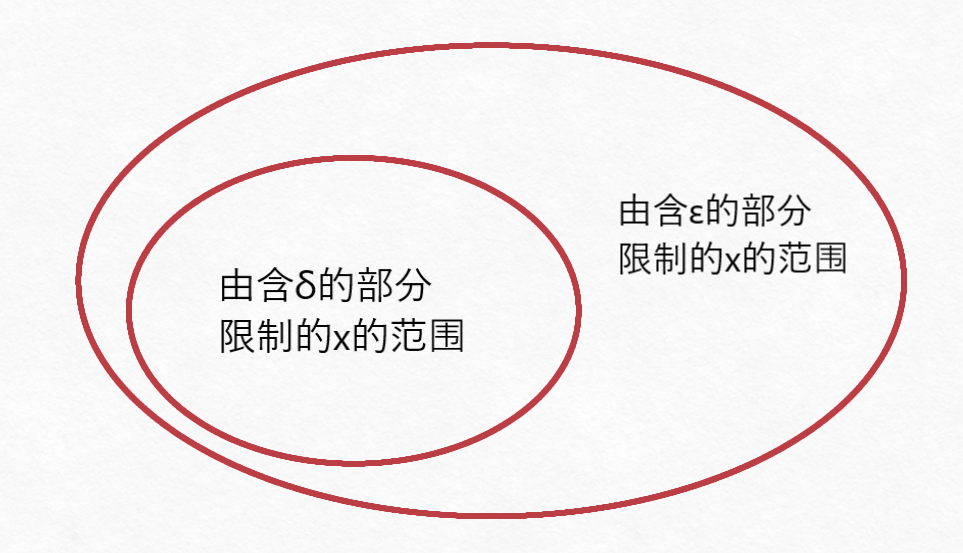
\includegraphics[scale=0.4]{1.png}
            \end{minipage}
        }
        \subfigure
        {
             \begin{minipage}[b]{.3\linewidth}
                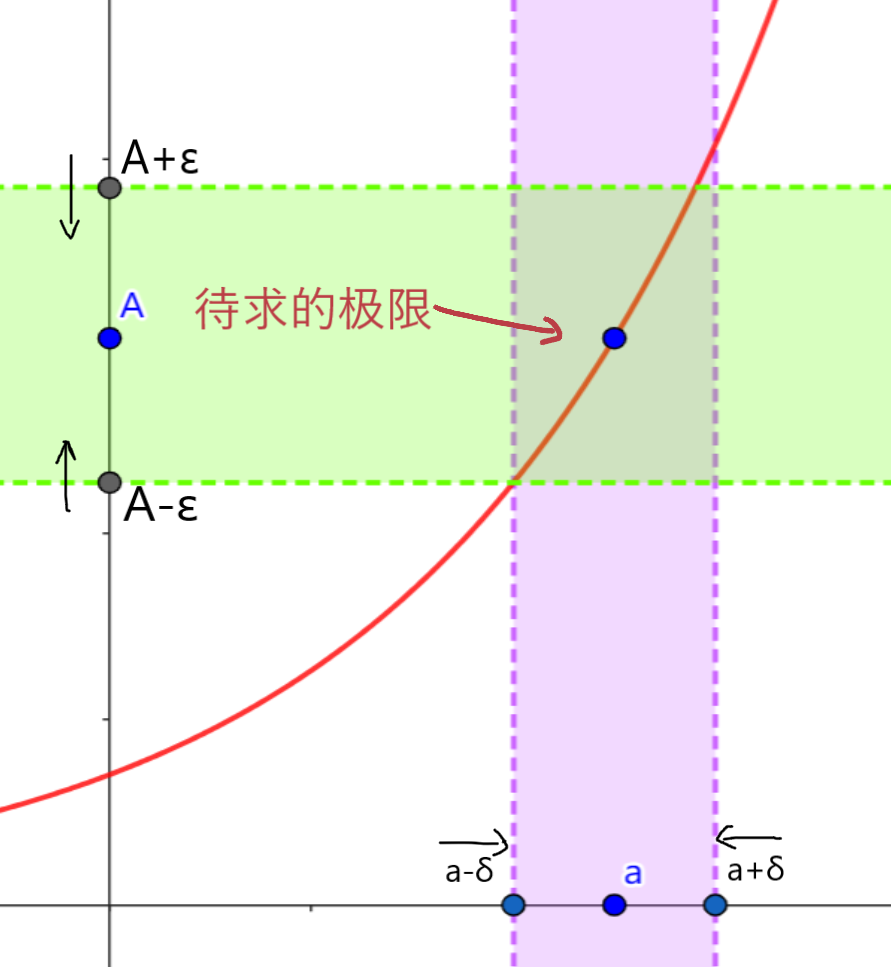
\includegraphics[scale=0.3]{2.png}
            \end{minipage}
        }
    \end{figure}
    
    \lishu 例题:证明$\lim_{x\rightarrow 1}\frac{x^2-1}{2x^2-x-1}=\frac{2}{3}$


    \(\)证明:首先,具象化$f(x)$和$A$,有$\left| f\left( x \right) -A \right|=\left| \frac{x^2-1}{2x^2-x-1}-\frac{2}{3} \right|$
    
    \(\)对等式右侧提公因式,化简得
    $$
    \left| \frac{x^2-1}{2x^2-x-1}-\frac{2}{3} \right|=\left| \frac{\left( x-1 \right) \left( x+1 \right)}{\left( x-1 \right) \left( 2x+1 \right)}-\frac{2}{3} \right|
    $$
    $$
    \ \ \ \ \ \ \ \ \ \ \ \ \ \ \ \ \ \ \ \ \ \ \ \ \ \ \ =\left| \frac{x+1}{2x+1}-\frac{2}{3} \right|=\left| \frac{x-1}{6x+3} \right|
    $$

    再然后,极限在$x=1$处取得,所以对于$x$的约束$|x-1|<\delta$,我们要求它总会使最终的结果$\left| \frac{x-1}{6x+3} \right|<\epsilon$。通过上述文章的分析,我们知道这实际上是对$\delta$的限制,事实上,我们把两个不等式联立来看,将会是这样的要求:
    $$\left| \frac{x-1}{6x+3} \right|<\frac{\delta}{\left| 6x+3 \right|}<\epsilon$$
    
    可见,一个关于$\delta-\epsilon$的约束就这样建立了起来。并且由题意,我们是在用$\epsilon$去限制$\delta$的取值。因为$\epsilon$处的逻辑用语是“$\forall$”(其意为“对于任意的$\epsilon$都有……”)而$\delta$的逻辑用语是“$\exists$”(其意为“存在至少一个$\delta$满足……”)。

    但是我们需要去掉其中包含x的部分,这样才是彻底的$\delta-\epsilon$的约束。但对于$x\in \mathbb{R}$的情况,因为分母的$\left| 6x+3 \right|\in \left( 0,+\infty \right)$,所以我们没办法轻易的消除这个部分,否则在它趋于0的时候,就要引发另一个极限问题了。但很显然我们要求的是$x\to 1$的极限,根本不是$x\in \mathbb{R}$的情况,而把x限制在$x\approx 1$附近的手段正是$\delta$,回过头来限制$\delta$的手段又是$\epsilon$。
    
    显然距离$x=1$太远的地方是不需要过多考虑的,至少思路上我们要尽可能把$\delta$取小,用以满足很小的$\epsilon$的约束。那么先随便划定一个范围,比如前后距离$\delta=1$的\ $0<x<2$,考虑$\delta<1$的时候,必然有$\left| 6x+3 \right|\in \left( 3,15 \right)$,那么$$\frac{\delta}{\left| 6x+3 \right|}<\underline{\ \frac{\delta}{3} <\epsilon\ }$$

    划线的部分正是我们要寻找的:由$\epsilon$限制的$\delta$的关系,我们找到了$\delta=3\epsilon$。于是我们可以写出结论:对于$\forall\epsilon$,都$\exists\delta=3\epsilon $,使得当$x$满足$0<\left| x-a \right|<\delta$时,都有$\left| f(x)-A \right|<\epsilon$成立。
    
    这个方程是在默认了$\delta<1$下成立的,$\delta<1$对应的约束应有$3\epsilon<1$。而关于如果存在$\delta>1$的情况,其实我们更关注$3\epsilon>1$,但是又考虑到,这个时候其实直接让$\delta=1$就可以使极限成立了,这和我们最开始的思路:让$\delta$尽可能小这点相吻合。\songti 

    证明的过程兜兜转转,我们为什么要绕那么多弯,进行那么麻烦的步骤呢?仔细观察我们解题时所做的所有事,都是在试图描述$\delta$和$\epsilon$变小的过程和关系,其中最难办的还是在处理一堆不等式上。注意到$f(x)=\frac{x^2-1}{2x^2-x-1}$在$x=1$处并没有定义,函数也没有取值,这导致我们用不了等号,所以麻烦的起源,其实是因为我们热衷于去寻找一个“不存在”的量。因为$x=1$并不能取到,所以我们引入了一个“距离量”$\delta$,用x处于1附近的邻域来代替$x=1$处的样子;因为$f(x)$在$f(1)$处也没有定义,所以我们引入了一个“$\epsilon$”,用“$f(1)$”附近的邻域代替不存在的$f(1)$进行运算,试图猜测和描述$f(1)$的性质。

    \begin{figure}[htbp]
        \centering
        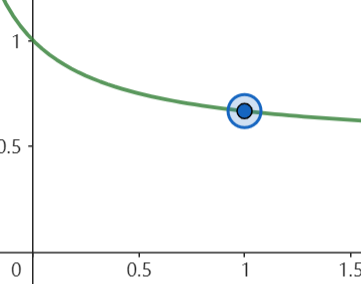
\includegraphics[scale=1]{3.png}
    \end{figure}
    
    求极限是一种预言的过程,它不意味着我们关注确切的取值,甚至可以不存在确切的取值,而是关注它的变化,大到整体函数的变化,小到一个邻域周围的变化。我们要做的其实是利用函数的性质,预言它的趋势和走向,我们取极限,看似求得的是最终的结果,但实际上我们真正想要的,是这个结果所反映的函数的性质。尤其是例如涉及无穷的极限,比如$e^{-x}$在x非常大的时候趋于0,这并非是说我们能找到0的取值,而是关注这个函数趋势的性质的一种表述。当然,这种性质可以展现为图像的形式,也可以体现为代数上的性质,这也是决定我们证明题中真正得以运算求解的原因。

    图像上来说,我们利用待求极限点的邻域,仔细审视这里的左右两侧,最后对该点进行预测。如果对于不是那么特殊的情况,类似于$f(x)=2x,\lim_{x\to1}2x=2=f(1)$。在一个很一般的函数上,找一些比较一般的点,那么我们取的极限往往只是函数值本身,并没有太多出入。
    
    这件事看似很普通,取值也是相同的,但是这个取值的由来是完全不一样的。其一源自于数值计算,其一来自于“预测”。如果我们通过一点的左右两侧的情况,成功预测了那个点的情况,就说明这个点和两侧的函数的性质是紧密相连的。所谓的预测吻合现实的性质,就称为函数的\underline{连续性}。“连”代表了前后性质的整体一致,“续”说明了彼可算此,此可推彼,函数的连续性,和函数的极限的意义,是密不可分的。

    对于不连续的情况,比如对于
    \begin{equation}
        \begin{split}f(x)=
            \begin{cases}
                1&,x>0\\
                0&,x=0\\
                -1&,x<0\\
            \end{cases}
        \end{split}
    \end{equation} 
    
    我们如果对于$x\to 0$处通过变化趋势的判断的话,用$x<0$的部分,取到的极限将会是$-1$。而利用$x>0$的部分预测,取到的极限将会是$1$,这显然和我们所定义的$f(0)=0$都是不同的。可见,一方面,极限的取值和函数值本身并无必然关系,这亦反映了我们取极限的过程绝非等同于计算,而是对性质的评估;另一方面,我们通过不同的预测手段,例如从$x=0$的左侧预测或者从右侧预测,取得的结果也可以不同。

    综上,总结为两点角度:①$x=0$处左右两侧的$f(x)$性质不同;②$x=0$处的$f(0)$与左右两侧的$f(x)$性质均不同。这样的函数就是不连续的函数,一方面是图像上显然就不能“连”起来,另一方面对于极限的角度,我们无法根据函数的各种性质去成功预测此处的函数值,反应了前后性质连续不上。

    接下来给出定义:对于任意一点$x=a$处,利用其“左侧”$x<a$部分的性质考虑极限,所求称为函数的左极限,记为$\lim_{x\to a^-}f(x)=A$,其中“$x\to a^-$”我们读作“x趋于a负”。同理,通过$x>a$的部分预言的极限,称为右极限,记为$\lim_{x\to a^+}f(x)=A$。对于左右极限不相等的情况,我们不能认为此处的极限是有定义的,需要额外强调待求的极限到底是左极限还是右极限。那么,如果左右极限相等,即$$\lim_{x\to a^-}f(x)=\lim_{x\to a^+}f(x)=A$$则说明极限$\lim_{x\to a}f(x)$存在且等于A。如果这个点的极限不仅存在,并且和函数值相等,即$$\lim_{x\to a}f(x)=f(a)$$则函数在该点连续。




\end{document}